\documentclass[12pt]{article}
\usepackage[margin=2cm]{geometry}
\usepackage{titling}
\usepackage[T1]{fontenc}
\usepackage{tabularx}
\usepackage{graphicx}
\usepackage{subcaption}
\usepackage{amsfonts}
\usepackage{amsmath}
\usepackage{amssymb}
\usepackage{algorithm}
\usepackage[noend]{algpseudocode}

\pretitle{\begin{center}\Huge\bfseries}
\posttitle{\par\end{center}\vskip 0.5em}
\preauthor{\begin{center}\Large}
\postauthor{\end{center}}
\predate{\par\large\centering}
\postdate{\par}

\title{Algorytmy Metaheurystyczne - lab 3}
\author{Jakub Musiał 268442}
\date{Styczeń 2024}

\begin{document}

\maketitle

\vspace*{2cm}

\section{Opis problemu}

Wyznaczyć przybliżenie optymalnego cyklu komiwojażera grafu pełnego używając algorytmu genetycznego.

\section*{Opis algorytmu}
    Schemat działania algorytmu genetycznego jest następujący:
    \begin{enumerate}
        \item Wyznaczenie populacji początkowej
        \item Selekcja "rodziców", którzy będą brali udział w procesie krzyżowania, z obecnej populacji
        \item Krzyżowanie - tworzenie "potomków" na podstawie genów "rodziców"
        \item Mutacja - z pewnym prawdopodobieństwem geny potomków mogą zostać poddane mutacji
        \item Powtórzenie kroków 2-4, jeśli nie osiągnięto warunku stopu
    \end{enumerate}

    \noindent\newline
    Poniżej przedstawiony jest pseudokod opisanego algorytmu.
    Użyte oznaczenia:
    \begin{itemize}
        \item $G$ - graf wejściowy
        \item $M$ - maksymalna liczba iteracji wyrażona jako procent liczby wierzchołków grafu
        \item $n_p$ - rozmiar populacji
        \item $crossover$ - metoda krzyżowania (zmienna funkcyjna)
        \item $p_m$ - prawdopodobieństwo mutacji
    \end{itemize}

    \noindent
    Dodatkowo by usprawnić działanie algorytmu zastosowałem wyspowy wariant algorytmu, w którym w tym samym czasie istnieje kilka odizolowanych populacji, w których wymiana informacji jest możliwa co $p$ pokoleń (w implementacji użyłem $p = 25$).

    \newpage

    \begin{algorithm}[h!]
    \caption{Genetic algorithm}\label{alg:genetic_algorithm}
    \begin{algorithmic}[1]
        \Procedure{$genetic\_algorithm$}{$G, M, n_p, crossover, p_m$}
            \State $P \gets generate\_population(G, n_p)$
                \Comment Initial population
            \State
            \For{$i \gets 1$ to $M \cdot |V_G|$}
                \State $p \gets select\_parents(P)$
                \State $P_n \gets \{\}$
                    \Comment Empty population
                \State
                \For{$i_p \gets 1$ to $|p|$}
                    \State $c_a \gets crossover(p[i_p].first, p[i_p].second)$
                    \State $c_b \gets crossover(p[i_p].second, p[i_p].first)$
                    \If{$random\_prob() < p_m$}
                        \State $c_a \gets mutate(c_a)$
                    \EndIf
                    \If{$random\_prob() < p_m$}
                        \State $c_b \gets mutate(c_b)$
                    \EndIf
                    \State $push(P_n, [c_a, c_b])$
                \EndFor
                \State
                \State $P \gets P_n$
                \State $\pi_b \gets argmin(P)$
                    \Comment Population member with the minimum weight
            \EndFor
            \State
            \Return $\pi_b$
        \EndProcedure
    \end{algorithmic}
    \end{algorithm}

\section*{Dobór parametrów}

    By określić najlepsze parametry przeprowadziłem eksperyment polegający na sprawdzeniu wyników
    kombinacji z losowej próbki wszystkich możliwych kombinacji poniżej określonych parametrów,
    a następnie znajdując taką, która generuje najmniejszy błąd względny.
    \newline

    \noindent \textbf{Badane parametry:}
    \begin{itemize}
        \item $M$ - maksymalna liczba iteracji (jako procent liczby wierzchołków grafu): $\{10, 25, 50\}$
        \item $n_p$ - rozmiar populacji: $\{50, 100\}$
        \item $crossover$ - metoda krzyżowania (zmienna funkcyjna): $\{simple, single\_point\}$
        \item $p_m$ - prawdopodobieństwo mutacji: $\{0.1, 0.2, 0.3\}$
    \end{itemize}

    \noindent Najlepszą znalezioną kombinacją parametrów jest:
    $$M = 50 \land n_p = 100 \land crossover = single\_point \text{ } \land p_m = 0.2$$
    dla której otrzymałem średni błąd względny $\delta = 0.126002$.

\newpage

\section*{Wyniki}

    Poniższa tabela oraz wykresy przedstawiają wyniki uzyskane dla wszystkich grafów testowych dla
    znalezionej kombinacji parametrów.

    \begin{table}[h!]
    \centering
    \begin{tabularx}{0.73\textwidth}{| c | c | c | c | c |}
        \hline
        Dane wejściowe & $|V|$ & $avg(w(TSC))$ & $min(w(TSC))$ & $w(TSC_{opt})$ \\
        \hline
        xqf131.tsp  & $131$  & $629$  & $599$  & $564$  \\
        xqg237.tsp  & $237$  & $1126$ & $1102$ & $1019$ \\
        pma343.tsp  & $343$  & $1522$ & $1482$ & $1368$ \\
        pka379.tsp  & $379$  & $1480$ & $1442$ & $1332$ \\
        bcl380.tsp  & $380$  & $1839$ & $1788$ & $1621$ \\
        pbl395.tsp  & $395$  & $1467$ & $1428$ & $1281$ \\
        pbk411.tsp  & $411$  & $1518$ & $1474$ & $1343$ \\
        pbn423.tsp  & $423$  & $1561$ & $1544$ & $1365$ \\
        pbm436.tsp  & $436$  & $1630$ & $1588$ & $1443$ \\
        xql662.tsp  & $662$  & $2847$ & $2818$ & $2513$ \\
        xit1083.tsp & $1083$ & $4079$ & $4073$ & $3558$ \\
        icw1483.tsp & $1483$ & $5067$ & $4944$ & $4416$ \\
        djc1785.tsp & $1785$ & $7054$ & $6917$ & $6115$ \\
        dcb2086.tsp & $2086$ & $7587$ & $7447$ & $6600$ \\
        pds2566.tsp & $2566$ & $8889$ & $8741$ & -      \\
        \hline
    \end{tabularx}
    \label{table:ga_results}
    \caption{Wyniki dla wszystkich danych wejściowych dla algorytmu genetycznego wraz z
    wagą optymalnych ścieżek}
    \end{table}

    \begin{table}[h!]
        \centering
        \begin{tabularx}{0.71\textwidth}{| c | c | c | c | c | c | c |}
            \hline
            Dane wejściowe & $|V|$ & $w_{C(MST)}$ & $avg_{LS}$ & $avg_{SA}$ & $avg_{TS}$ & $avg_{GA}$ \\
            \hline
            xqf131.tsp  &$131$  & $742$  & $621$  & $576$  & $614$  & $629$  \\
            xqg237.tsp  &$237$  & $1424$ & $1118$ & $1049$ & $1108$ & $1126$ \\
            pma343.tsp  &$343$  & $1876$ & $1497$ & $1380$ & $1485$ & $1522$ \\
            pka379.tsp  &$379$  & $1799$ & $1450$ & $1341$ & $1447$ & $1480$ \\
            bcl380.tsp  &$380$  & $2337$ & $1817$ & $1663$ & $1802$ & $1839$ \\
            pbl395.tsp  &$395$  & $1893$ & $1456$ & $1312$ & $1431$ & $1467$ \\
            pbk411.tsp  &$411$  & $1930$ & $1489$ & $1380$ & $1485$ & $1518$ \\
            pbn423.tsp  &$423$  & $1921$ & $1533$ & $1403$ & $1528$ & $1561$ \\
            pbm436.tsp  &$436$  & $2095$ & $1629$ & $1481$ & $1611$ & $1630$ \\
            xql662.tsp  &$662$  & $3692$ & $2822$ & $2583$ & $2816$ & $2847$ \\
            xit1083.tsp &$1083$ & -      & $4021$ & $3655$ & $3936$ & $4079$ \\
            icw1483.tsp &$1483$ & -      & $4986$ & $4532$ & $4886$ & $5067$ \\
            djc1785.tsp &$1785$ & -      & $6878$ & $6273$ & $6837$ & $7054$ \\
            dcb2086.tsp &$2086$ & -      & $7463$ & $6810$ & $7342$ & $7587$ \\
            pds2566.tsp &$2566$ & -      & $8695$ & $7898$ & $8685$ & $8889$ \\
            \hline
        \end{tabularx}
        \label{table:results_comparison}
        \caption{Porównanie wyników dla wszystkich badanych algorytmów}
        \end{table}

        \newpage

        \begin{figure}[htpb]
        \centering
            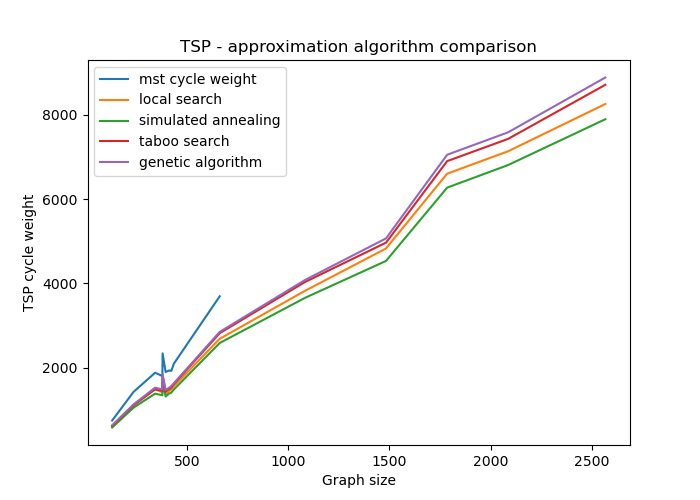
\includegraphics[width=0.7\linewidth]{img/algs.png}
            \caption{Porównanie wyników dla wszystkich badanych algorrytmów}
        \end{figure}

        \noindent
        Na podstawie powyższej tabeli oraz wykresu możemy zauważyć, że dla zadanego problemu najlepsze wyniki zwróciła metoda symulowanego wyżarzania.

        \newpage

        \begin{figure}[htpb]
        \centering
            \begin{subfigure}[b]{0.475\textwidth}
                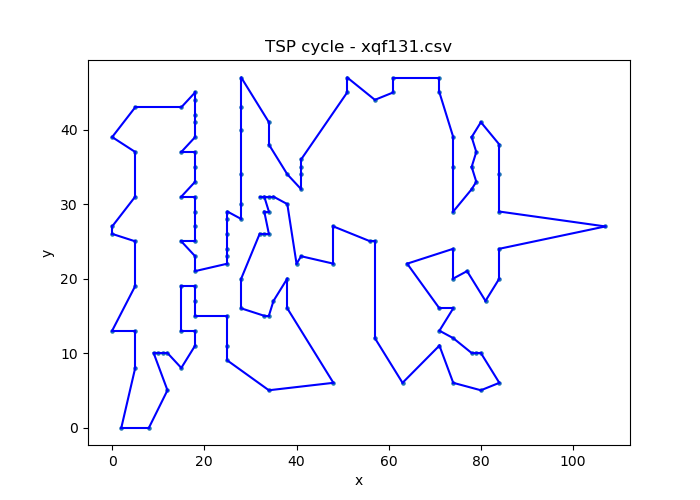
\includegraphics[width=\linewidth]{img/xqf131.png}
            \end{subfigure}
            \hfill
            \begin{subfigure}[b]{0.475\textwidth}
                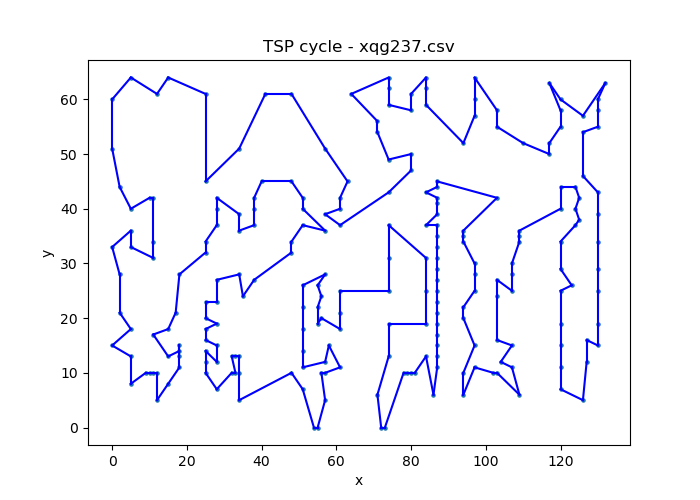
\includegraphics[width=\linewidth]{img/xqg237.png}
            \end{subfigure}
            \begin{subfigure}[b]{0.475\textwidth}
                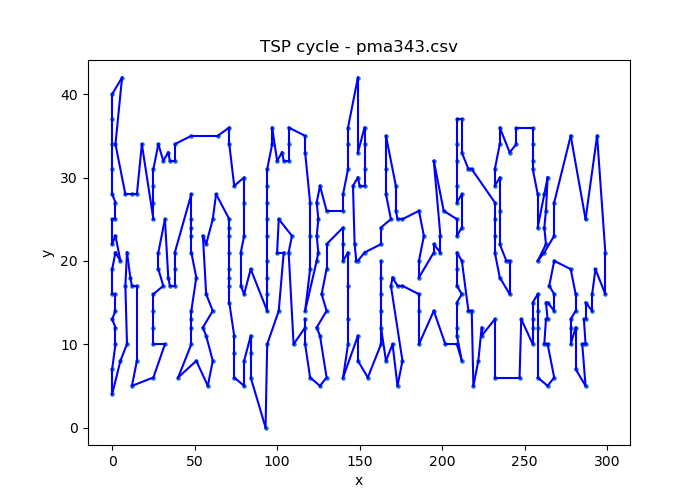
\includegraphics[width=\linewidth]{img/pma343.png}
            \end{subfigure}
            \hfill
            \begin{subfigure}[b]{0.475\textwidth}
                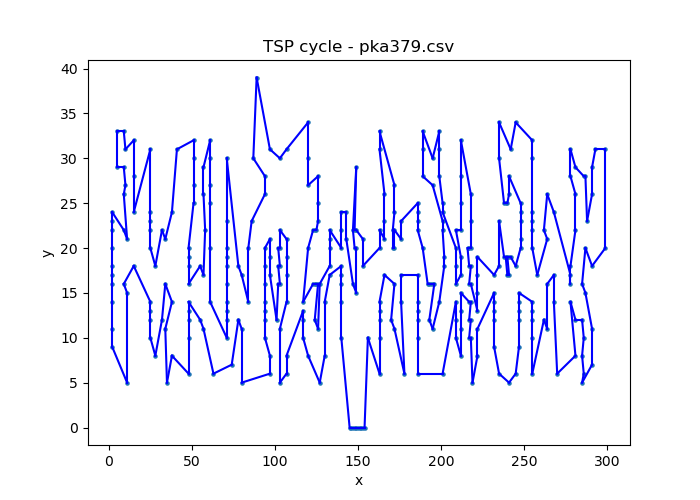
\includegraphics[width=\linewidth]{img/pka379.png}
            \end{subfigure}
            \begin{subfigure}[b]{0.475\textwidth}
                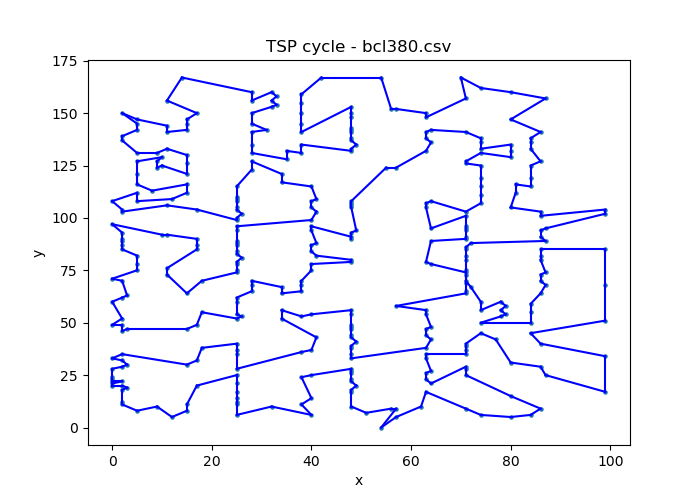
\includegraphics[width=\linewidth]{img/bcl380.png}
            \end{subfigure}
            \hfill
            \begin{subfigure}[b]{0.475\textwidth}
                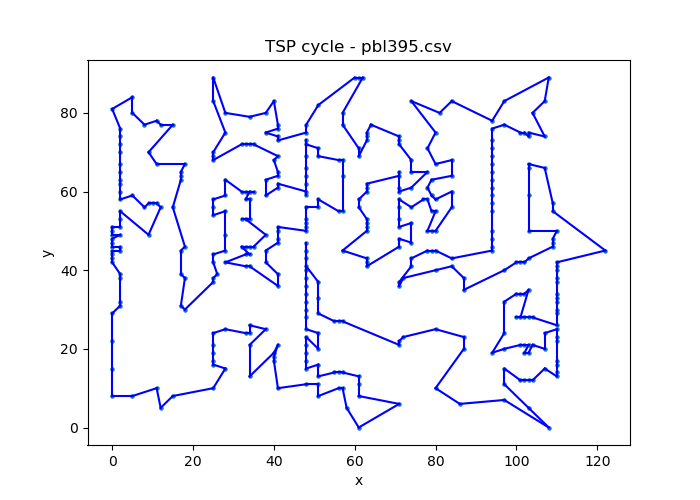
\includegraphics[width=\linewidth]{img/pbl395.png}
            \end{subfigure}
            \begin{subfigure}[b]{0.475\textwidth}
                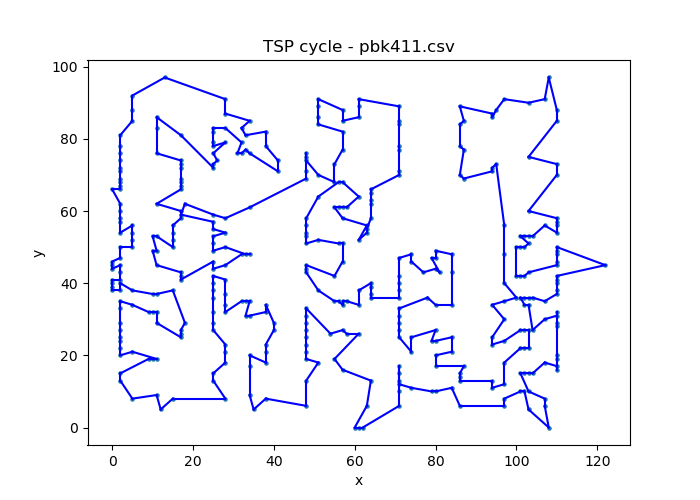
\includegraphics[width=\linewidth]{img/pbk411.png}
            \end{subfigure}
            \hfill
            \begin{subfigure}[b]{0.475\textwidth}
                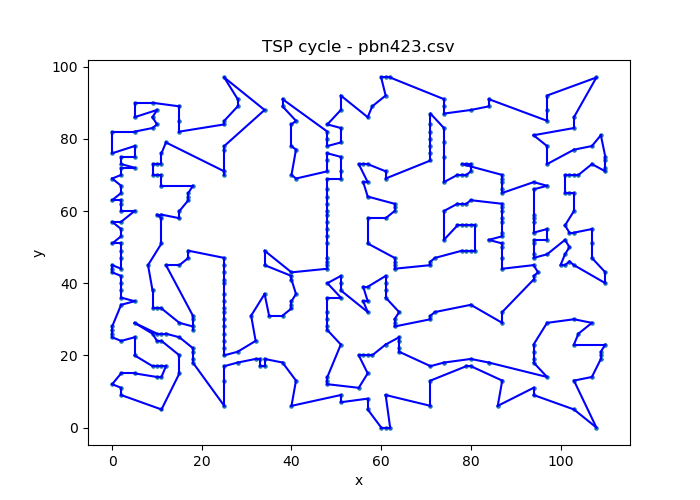
\includegraphics[width=\linewidth]{img/pbn423.png}
            \end{subfigure}
        \end{figure}

        \begin{figure}[htpb]
        \centering
            \begin{subfigure}[b]{0.475\textwidth}
                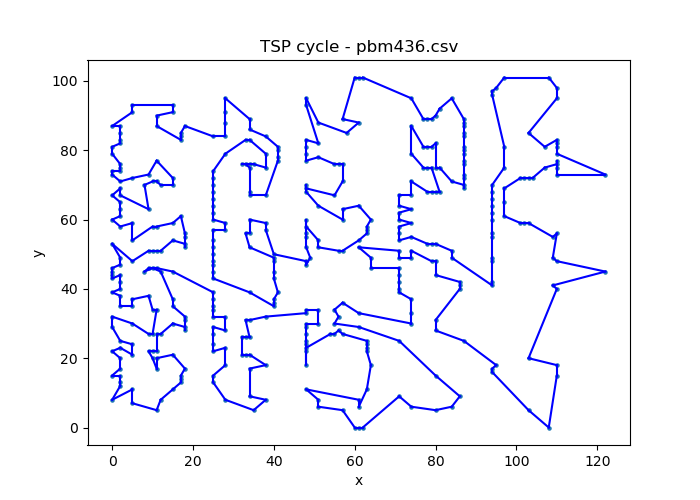
\includegraphics[width=\linewidth]{img/pbm436.png}
            \end{subfigure}
            \hfill
            \begin{subfigure}[b]{0.475\textwidth}
                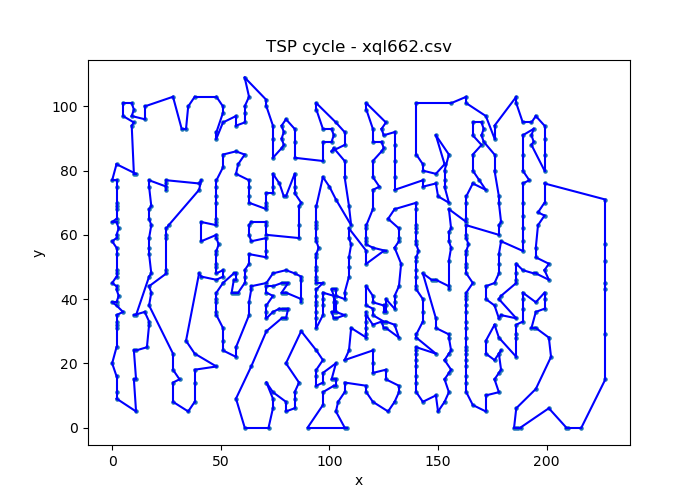
\includegraphics[width=\linewidth]{img/xql662.png}
            \end{subfigure}
            \begin{subfigure}[b]{0.475\textwidth}
                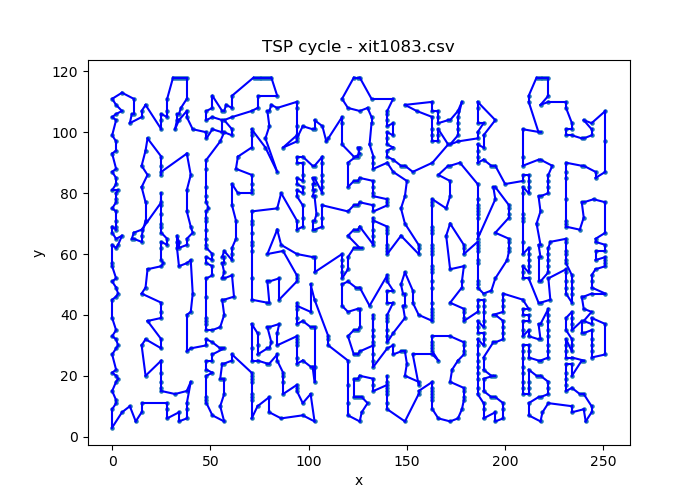
\includegraphics[width=\linewidth]{img/xit1083.png}
            \end{subfigure}
            \hfill
            \begin{subfigure}[b]{0.475\textwidth}
                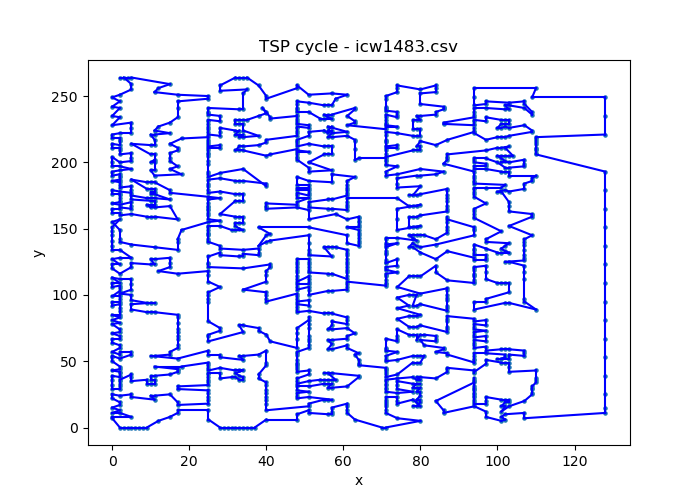
\includegraphics[width=\linewidth]{img/icw1483.png}
            \end{subfigure}
            \begin{subfigure}[b]{0.475\textwidth}
                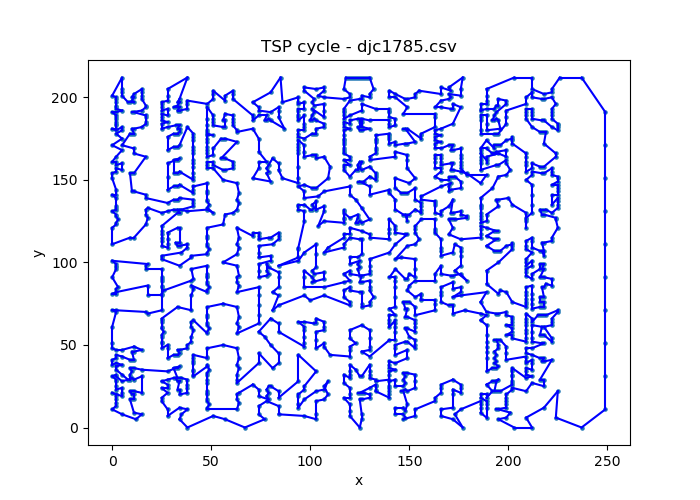
\includegraphics[width=\linewidth]{img/djc1785.png}
            \end{subfigure}
            \hfill
            \begin{subfigure}[b]{0.475\textwidth}
                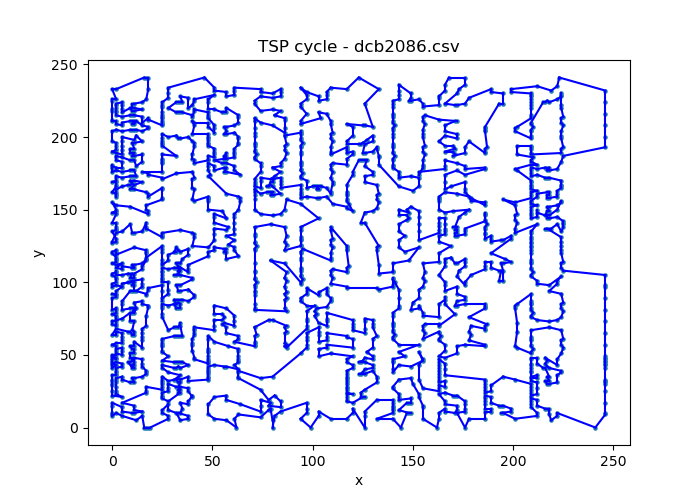
\includegraphics[width=\linewidth]{img/dcb2086.png}
            \end{subfigure}
            \begin{subfigure}[b]{0.475\textwidth}
                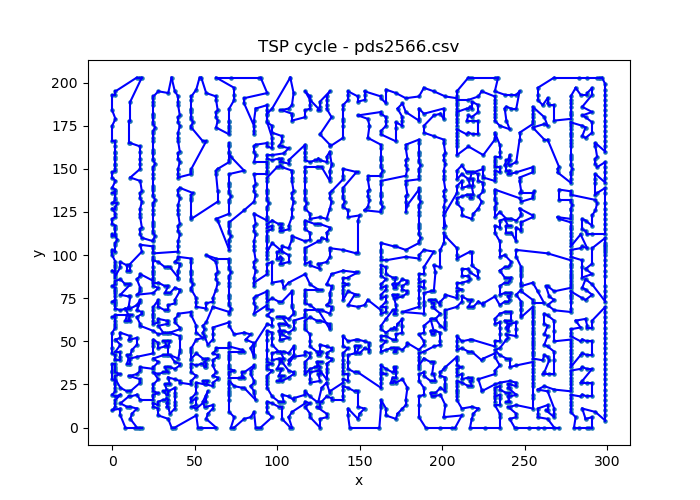
\includegraphics[width=\linewidth]{img/pds2566.png}
            \end{subfigure}
            \caption{Genetic algoritm: wizualizacja wyznaczonych cykli komiwojażera}
        \end{figure}

\end{document}
